\documentclass{article}

%............Inicia Preambulo.......................
\usepackage{graphicx}
\usepackage{float}
\usepackage[utf8]{inputenc}
\usepackage[shortlabels]{enumitem}
\usepackage{textcomp}
\usepackage{multicol}
\usepackage{caption}
\usepackage[spanish]{babel}
\usepackage[total={17.5cm, 23cm}, top=2cm, left=2cm]{geometry}
\usepackage{esvect}
\usepackage[font=footnotesize]{caption}

\spanishdecimal{.}
\parindent 0cm

%.............Fin de Preambulo........................

\begin{document}

\begin{center}
{\Large \textbf{Universidad Autónoma de Coahuila}}
\end{center}

\begin{center}
{\large Facultad de Ciencias Físico-Matemáticas}
\end{center}

%Materia
\begin{center}
{\large Metodos Numericos}
\end{center}

%Título
\begin{center}
{\large Metodo de Muller}
\end{center}

%Fecha
\begin{center}
{\large 29 de Noviembre del 2019}
\end{center}

%Autor
\begin{center}
{\large José Antonio Olveda García}
\end{center}

\vspace{5mm}

\begin{multicols}{2}

\section{Objetivo}
\label{sec:obj}
  El objetivo de este metodo es demostrar la utilidad de uno de los metodos de busca de raices mas escenciales como lo es muller, asi como las ventajas y desventajas que este presenta.
\section{Introduccion}
\label{sec:intro}
Recuérdese que el método de la secante obtiene raíces estimando una proyección de una línea recta en el eje de las x a través de dos valores de la función.
\\
El método de Müller toma un punto de vista similar, pero proyecta una parábola a través de tres puntos.
\\
El método consiste en obtener los coeficientes de tres puntos de la parábola. 
\\
Estos coeficientes pueden ser sustituidos en la fórmula cuadrática para obtener el punto donde la parábola intercepta el eje x; es decir, la raíz estimada

\section{Metodologia}
\label{sec:Met}


La aproximación es fácil de escribir en forma conveniente como la ecuación de una parábola:

\begin{equation}
f_{2}(x)=a(x-x_{2})^{2}+b(x-x_{2})+c
\end{equation}
Se busca esta parábola para intersectar los tres puntos $[x_{0},f(x_{0})], [x_{1},f(x_{1})],[x_{2},f(x_{2})]$
Los coeficientes de la ecuación pueden evaluarse al sustituir cada uno de esos tres puntos para dar:
\begin{center}
$f(x_{0})=a(x_{0}-x_{2})^{2}+b(x_{0}-x_{2})+c
$
\\
$f(x_{1})=a(x_{1}-x_{2})^{2}+b(x_{1}-x_{2})+c$
\\
$f(x_{2})=a(x_{2}-x_{2})^{2}+b(x_{2}-x_{2})+c$
\end{center}

El cual puede resolverse con ayuda de las siguientes relaciones algebraicas:
\begin{equation}
h_{0}=x_{1}-x_{0}
\end{equation}
\\
\begin{equation}
h_{1}=x_{2}-x_{1}
\end{equation}
\\
\begin{equation}
a_{1}= \frac{f(x_{1})-f(x_{2})}{x_{1}-x_{0}}
\end{equation}
\\
\begin{equation}
b_{1}= \frac{f(x_{2})-f(x_{1})}{x_{2}-x_{1}}
\end{equation}
Para finalmente hallar el valor de los coeficientes de la parábola:
\begin{equation}
a= \frac{b-a}{h1+h0}
\end{equation}
\\
\begin{equation}
b=ah_{1}+ a_{1}
\end{equation}
\\
\begin{equation}
c=f(x_{2})
\end{equation}
Una vez hallados a,b y c se utiliza la ecuación cuadrática para hallar el intercepto con el eje x, el cual sera la próxima aproximación.
\begin{equation}
x_{3}=x_{2}- \frac{2c}{b\pm \sqrt[2]{b^{2}-4ac}}\end{equation}

El signo del determinante se selecciona de tal manera que el denominador sea el más grande posible, esto garantiza que se escoja el intercepto $X_{3}$ más cercano a $X_{2}$

Una de las ventajas del método radica en que, al usar la fórmula cuadrática, es capaz de hallar raíces complejas. La principal desventaja es que en cada iteración se descarta una posible raíz de la parábola sin conocer la naturaleza de la misma.
\section{Ejemplo}
\label{sec:Ejem}
Encuentre las raices de $$x^{2}-25$$
con los puntos $x_{0}$, $x_{1}$ y $x_{2}$ evualuando $$f_{x_{0}}= (7)^{2}-25=24$$
$$f_{x_{1}}=(8)^{2}-25=39$$
$$f_{x_{2}}=(9)^{2}-25=56$$

$$e_{0}=f_{x_{0}}-f_{x_{2}}=-32$$
$$e_{1}=f_{x_{1}}-f_{x_{2}}=-17$$

$$h_{1}=x_{1}-x_{2}=-1$$
$$h_{2}=x_{0}-x_{2}=-2$$
$$w=h_{1}h_{2}^{2}-h_{1}^{2}h_{2}=-2$$
$$a=\frac{e_{0}h_{1}-e_{1}h_{2}}{w}=1$$
$$b=\frac{e_{1}h_{2}^{2}-h_{1}^{2}e_{0}}{w}=18$$

Por lo tanto las constantes serian $a=1$, $b=18$ y $c=56$
$$x_{3}=-5$$
$$x_{3}=5$$
siendo las raices del aplicar la formula estimada en muller

\section{Ventajas y Desventajas}
\label{sec:Ven}
\textbf{Ventajas}
\\
1. Por medio de este metodo se encuentran tanto raices reales como complejas.
\\
\\
\textbf{Desventajas}
\\
1.Se escoge el signo que coincida en el signo de "b", esta eleccion da como resultado el denominador mas grande, lo que dara la raiz estimada mas cercana a $x_{2}$
\\
2. Una vez que se determino $x_{3}$ el proceso se repite, eso trae que un valor es descartado.




\section{Implementacion del programa}
\label{sec:Imp}
El programa, genera una funcion llamada muller, el cual declara las ecuaciones determinadas, generando asi dicho metodo, al igual que los programas anteriores, este tambien genera una grafica para que el usuario pueda ver que es lo que sucede con la funcion ingresada
\begin{figure}[H]
\centering
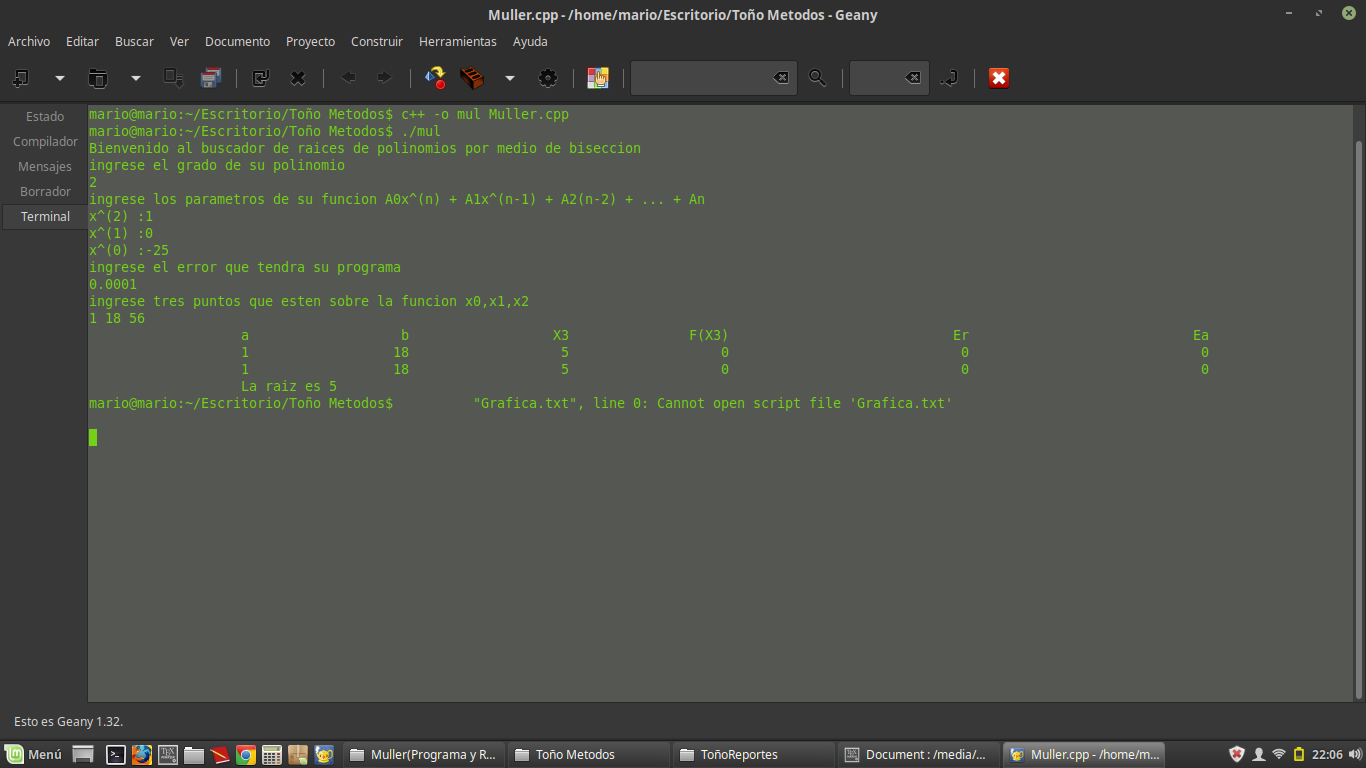
\includegraphics[scale=.125]{Muller.png}
\caption{Programa del metodo de muller}
\end{figure}
La funcion designada fue $x^{2}-25$ la cual corta en los puntos -5 y 5; debido a que muller es un metodo de la secante, este tomara la raiz que mas se aproxime a los puntos declarados, sin embargo en caso de obtenerse valores negativos en la raiz, se deja como ejercicio debido a que la programacion con respecto a los numeros complejos obtiene una mayor dificultad de resolucion.



\end{multicols}

\end{document}